%%=============================================================================
%% Proof of concept
%%=============================================================================
\graphicspath{ {./graphics/} }
\chapter{\IfLanguageName{dutch}{Proof Of Concept}{Proof Of Concept}}%

In dit hoofdstuk wordt de proof of concept uitgewerkt. De recent verkregen informatie wordt hierbij omgezet in de praktijk. De Proof Of Concept zal een beeld vormen van de oplossing voor het gestelde probleem. Als eerst zal er gekeken worden naar de gebruikte netwerkopstelling binnen Azure.
Vervolgens zal de gebruikte infrastructuur aan bod komen. Daarnaast zal er dieper worden ingegaan op Ansible en de bijhorende playbooks die zorgen voor de configuratie van de firewall. Verder wordt er gekeken naar de uitwerking van het powershell script dan instaat voor het uitvoeren van controles op de ingevoerde data door de klant. Dit script zal alle zaken die hiervoor werden besproken samenbrengen tot 1 werkende geheel. 

\newpage

\section{Netwerkopstelling}
De netwerkopstelling die gebruikt wordt voor de Proof of Concept bestaat uit 2 virtuele machines elk in hun eigen subnet respectievelijk. In het eerste subnet met netwerkadres 172.22.2.0 bevindt zich een virtuele machine met het adres 172.22.2.5. Op deze machine staat een apache webserver geïnstalleerd. In het tweede subnet met netwerkadres 172.22.1.0 bevindt zich een virtuele machine met het adres 172.22.1.5. Deze machine zal dienen als host. Tussen deze twee subnets bevindt zich een firewall in de vorm van een Network Virtual Appliance (NVA) van Fortinet. Deze maakt gebruik van drie interfaces. Elk subnet is verbonden met één van deze interfaces. De derde interface is verbonden met de buitenwereld. Deze netwerkopstelling zorgt voor een ideale testomgeving. De mogelijkheid voorzien dat de host de webserver kan bereiken aan de hand van geautomatiseerde firewallrules met behulp van Ansible waarop, controle is uitgevoerd doormiddel van een powershell script, is het uitendelijke doel van deze Proof of Concept. In het werkveld zal deze opstelling complexer zijn dan wat hier wordt opgebouwd. Voor dit onderzoek is het voldoende om het simpel te houden. Dit is een perfecte manier om aan te tonen dat de onderzoeksvraag beantwoord wordt. 
\newline

\begin{tabularx}{0.8\textwidth} { 
  | >{\centering\arraybackslash}X 
  | >{\centering\arraybackslash}X 
  | >{\centering\arraybackslash}X
  | >{\centering\arraybackslash}X | }
 \hline
 Naam & Subnet & Adres & Firewall interface \\
 \hline
 Host  & 172.22.1.0  & 172.22.1.5 & 172.22.1.4 \\
\hline
 Webserver  & 172.22.2.0  & 172.22.2.5  & 172.22.2.4 \\
\hline
\end{tabularx}
\subsection{Topologie}

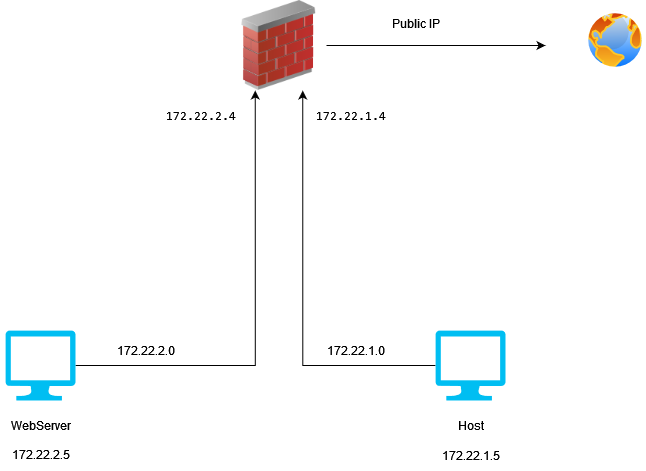
\includegraphics[width=100mm]{bachproef/graphics/topologie.drawio.png}
\newpage
\section{Infrastructuur}
In dit onderdeel wordt besproken welke software , tools etc. gebruikt worden voor het opstellen van de Proof of Concept. Ook wordt er besproken wat er gebruikt wordt bij het uitwerken van de eerste versies en welke problemen dit met zich meebrengt om uiteindelijk niet voor die bepaalde optie te kiezen. Het is de bedoeling dat de infrastructuur snel en makkelijk opgezet kan worden door eender wie, zonder dat er veel extra software geïnstalleerd dient te worden. 
\subsection{Manueel?}
Als eerste werd er gekeken naar een oplossing waarbij er manueel een linux virtuele machine werd opgezet. Hierop werd de nodige software (Ansible, ...) geïnstalleerd en al de benodigdheden geconfigureerd. Het werd al snel duidelijk dat dit een zeer omslachtige manier van werken was. Er was geen makkelijke manier om met een shared folder te werken. De enige manier om deze configuratie van de virtuele machine te delen was door het nemen van een image en deze te versturen. Deze bestanden kunnen groot zijn en zijn bijgevolg niet makkelijk te verdelen. Het was ook niet mogelijk om vanop afstand gemakkelijk de configuratie van de virtuele machine te gaan aanpassen. Hiervoor moest je steeds rechtstreeks inloggen op de machine en de juiste configuratie bestanden zoeken en aanpassen. Er was dus nood aan een vorm van automatisatie om zaken makkelijker te configureren. Het moest ook makkelijker door te geven zijn aan bijvoorbeeld een collega, zonder dat deze hiervoor een groot bestand moest binnenhalen. 
\subsection{Vagrant?}
Om de problemen op te lossen die kwamen kijken bij het manueel opstellen, werd er gebruik gemaakt van Vagrant. Dit is een handige tool voor de automatisatie en installatie van virtuele machines met een specifieke configuratie. Voor deze Proof of Concept werd er een virtuele machine opgezet met Vagrant waarop de Ansible software werd geïnstalleerd. Dit zorgde voor enkele problemen. Het was niet mogelijk voor de virtuele machine om een verbinding op te zetten met de firewall om hierop zaken te gaan uitvoeren met behulp van Ansible. Met Vagrant werken zou er bijgevolg ook tot leiden dat er allerlei zaken zouden moeten geïnstalleerd worden op de lokale host. Dit zorgt ervoor dat het niet zo vanzelfsprekend is om dit door te geven aan een collega. Hiervoor zou documentatie geschreven horen te worden om de werking van alles te begrijpen. Dit leidde tot de conclusie dat dit een te omslachtige manier van werken is , dit kon dus makkelijker. 
\newpage

\subsection{Docker!}
Aangezien Vagrant niet meteen gezien wordt als de beste oplossing, is er nood aan een alternatief. Wanneer er nood is aan een oplossing waarbij snel en efficiënt een instantie van een virtuele machine moet worden opgezet , waarbij flexibiliteit belangrijk is, blijkt Docker een goeie oplossing. De mogelijkheid om de configuratie op dockerhub te plaatsen zorgt voor een makkelijke distributie van de opstelling. Docker is bijgevolg de enige software die nodig is voor het opstellen en gebruiken van de gehele infrastructuur. Het installeren van deze software kan op twee manieren. In het geval van een Windows machines kan dit op twee verschillende manieren gebeuren. Dit kan enerzijds via de command line interface of anderzijds via een .exe bestand. Op Linux machines kan dit enkel via de command line interface. Hiervoor kan de documentatie van Docker geraadpleegd worden via \url{ https://www.docker.com/}. \newline

Docker maakt gebruik van een eigen bestandsformaat, namelijk een dockerfile. Deze dockerfile wordt gebruikt voor het configureren van instanties van een virtuele machine. Deze instanties worden containers genoemd. Deze containers bevatten enkel de software en functionaliteiten die meegegeven worden in de dockerfile. \newline

Hieronder worden enkele lijnen getoond afkomstig uit de dockerfile die gebruikt werd voor de opbouw van de Proof of Concept. 

\begin{verbatim}
FROM ubuntu:22.04

RUN apt-get update && apt-get upgrade -y
RUN apt-get -y install python3 python3-nacl python3-pip libffi-dev vim

COPY ./credentials /root/.azure/
COPY ./azureProfile.json /root/.azure/
\end{verbatim}
Het eerste wat meteen opvalt is de manier waarop het bestand is opgebouwd. Een Dockerfile is makkelijk leesbaar. Zo wordt er gebruik gemaakt van verschillende keywords. het keyword "FROM" wordt gebruikt om te definiëren welke Operating system er gebruikt zal worden. In dit voorbeeld is de container een Linux machine die gebruik maakt van de Ubuntu versie 22.04 distributie. Verder wordt er gebruik gemaakt van het keyword "RUN". Na dit keyword volgt er steeds een commando dat uitgevoerd dient te worden op de command line interface. In dit voorbeeld worden er verschillende packages , zoals python , pip , vim ,... geïnstalleerd bij het bouwen van de container. Het keyword "COPY" wordt daarnaast gebruikt voor het kopiëren van bestanden, afkomstig van de lokale machine,naar de container. 

%%=============================================================================
%% Methodologie
%%=============================================================================

\chapter{\IfLanguageName{dutch}{Methodologie}{Methodology}}%
\label{ch:methodologie}
Dit onderzoek zal in verschillende delen verlopen. In hoofdstuk twee werd er vooral informatie vergaard om het probleem zo goed mogelijk te begrijpen. Deze informatie werd verkregen aan de hand van een relevante literatuurstudie. Ook zal er beroep gedaan worden op interviews met belanghebbenden om op deze manier een requirements-analyse te kunnen uitvoeren. Dit zal ervoor zorgen dat er een optimale oplossing komt voor het beschreven probleem. De informatie wordt vervolgens gebruikt voor het opmaken van een Proof-of-Concept, waarin alle informatie zal toegepast worden in de praktijk. Dit Proof-of-Concept zal uiteindelijk ook het eindproduct zijn, waarin de oplossing van het probleem wordt weergegeven. Hierover zal ook een presentatie gegeven worden. Voor dit onderdeel wordt er beroep gedaan op communicatie met de copromoter en het bedrijf waarvoor dit onderzoek wordt uitgevoerd. Hiervoor zal een uitgebreide verzameling van software en hardware nodig zijn. Zo zal het mogelijk moeten zijn om gebruik te maken van alle Microsoft Azure features voor een zo'n specifiek mogelijke oplossing. Op deze manier kan er een realistisch scenario worden opgebouwd. Verder zal er ook eventueel beroep gedaan worden op een webapplicatie waarmee het mogelijk is firewall regels in te geven. Dit zal een zeer simpele applicatie zijn, geschreven in JavaScript. Deze applicatie is essentieel voor het oplossen van het gegeven probleem. Het is de bedoeling dat een klant aan de hand van een webapplicatie firewall regels kan doorsturen naar een firewall. Deze regels zullen worden opgenomen in een JSON-file. Op deze manier kan deze makkelijk worden geïmplementeerd in een script. Deze scripts worden gemaakt met Ansible in combinatie met een andere tool.  
Het zou kunnen dat tijdens het uitvoeren van het effectief onderzoek een betere oplossing wordt gevonden.
Concreet wordt er een Azure netwerk opgezet met een Network Virtual Appliance van het merk Fortigate. Op dit netwerk zal dan ook een webapplicatie draaien. Vervolgens worden er templates gebouwd, in verschillende Infrastructure as Code tools, voor het deployen van de gewenste firewall regels. Vervolgens zal er ook gekeken worden of deze manier van werken ook toegepast kan worden op een firewall van een andere vendor zoals Cisco. Voor dit onderdeel wordt ongeveer 40 uur geschat. Ten slotte worden de resultaten geanalyseerd en samen gebundeld in een concrete conclusie. 
%% TODO: Hoe ben je te werk gegaan? Verdeel je onderzoek in grote fasen, en
%% licht in elke fase toe welke stappen je gevolgd hebt. Verantwoord waarom je
%% op deze manier te werk gegaan bent. Je moet kunnen aantonen dat je de best
%% mogelijke manier toegepast hebt om een antwoord te vinden op de
%% onderzoeksvraag.



